\documentclass[10pt]{article}

%%%%%%%%%%%%%%Include Packages%%%%%%%%%%%%%%%%%%%%%%%%%%
\usepackage{xcolor}
\usepackage{mathtools}
\usepackage[legalpaper, margin=1in]{geometry}
\usepackage{amsmath}
\usepackage{amssymb}
\usepackage{paralist}
\usepackage{rsfso}
\usepackage{amsthm}
\usepackage{wasysym}
\usepackage[inline]{enumitem}   
\usepackage{hyperref}
\usepackage{tocloft}
%%%%%%%%%%%%%%%%%%%%%%%%%%%%%%%%%%%%%%%%%%%%%%%%%%%%%%%%

%%%%%%%%%%%%%%%%%Theorem environments%%%%%%%%%%%%%%%%%%%
\newtheoremstyle{break}
  {\topsep}{\topsep}%
  {\itshape}{}%
  {\bfseries}{}%
  {\newline}{}%
\theoremstyle{break}
\theoremstyle{break}
\newtheorem{axiom}{Axiom}
\newtheorem{thm}{Theorem}[section]
\newtheorem{lem}{Lemma}[thm]
\newtheorem{prop}[thm]{Proposition}
\newtheorem{corL}{Corollary}[lem]
\newtheorem{corT}[lem]{Corollary}
\newtheorem{defn}{Definition}[corL]
\newenvironment{indEnv}[1][Proof]
  {\proof[#1]\leftskip=1cm\rightskip=1cm}
  {\endproof}
%%%%%%%%%%%%%%%%%%%%%%%%%%%%%%%%%%%%%%%%%%%%%%%%%%%%%%

%%%%%%%%%%%%%%%%%%%%%%%Integral%%%%%%%%%%%%%%%%%%%%%%%
\def\upint{\mathchoice%
    {\mkern13mu\overline{\vphantom{\intop}\mkern7mu}\mkern-20mu}%
    {\mkern7mu\overline{\vphantom{\intop}\mkern7mu}\mkern-14mu}%
    {\mkern7mu\overline{\vphantom{\intop}\mkern7mu}\mkern-14mu}%
    {\mkern7mu\overline{\vphantom{\intop}\mkern7mu}\mkern-14mu}%
  \int}
\def\lowint{\mkern3mu\underline{\vphantom{\intop}\mkern7mu}\mkern-10mu\int}
%%%%%%%%%%%%%%%%%%%%%%%%%%%%%%%%%%%%%%%%%%%%%%%%%%%%%%



\newcommand{\R}{\mathbb{R}}
\newcommand{\N}{\mathbb{N}}
\newcommand{\Z}{\mathbb{Z}}
\newcommand{\Q}{\mathbb{Q}}
\newcommand{\A}{\mathcal{A}}
\newcommand{\D}{\mathcal{D}}
\newcommand{\J}{\mathcal{J}}
\newcommand{\T}{\mathcal{T}}
\newcommand{\Td}{\mathcal{T}_d}
\newcommand{\C}{\mathcal{C}}
\newcommand{\M}{\mathcal{M}}
\newcommand{\Complex}{\mathbb{C}}
\newcommand{\Power}{\mathcal{P}}
\newcommand{\ee}{\cdot 10}
\newcommand{\spa}{\text{span}}
\newcommand{\vmat}[1]{\begin{vmatrix} #1 \end{vmatrix}}
\newcommand{\rref}{\xrightarrow{\text{row\ reduce}}}


\newcommand{\note}{\color{red}Note: \color{black}}
\newcommand{\remark}{\color{blue}Remark: \color{black}}
\newcommand{\example}{\color{green}Example: \color{black}}
\newcommand{\exercise}{\color{green}Exercise: \color{black}}




%%%%%%%%%%%%table of contents%%%%%%%%%%%%%%%%%%%%%%%%%%%%
\cftsetindents{section}{0em}{2em}
\cftsetindents{subsection}{0em}{2em}

\renewcommand\cfttoctitlefont{\hfill\Large\bfseries}
\renewcommand\cftaftertoctitle{\hfill\mbox{}}

\setcounter{tocdepth}{2}
%%%%%%%%%%%%%%%%%%%%%%%%%%%%%%%%%%%%%%%%%%%%%%%%%%%%%%%%%


%%%%%%%%%%%%%%%%%%%%%Footnotes%%%%%%%%%%%%%%%%%%%%%%%%%%%
\newcommand\blfootnote[1]{%
  \begingroup
  \renewcommand\thefootnote{}\footnote{#1}%
  \addtocounter{footnote}{-1}%
  \endgroup
}
%%%%%%%%%%%%%%%%%%%%%%%%%%%%%%%%%%%%%%%%%%%%%%%%%%%%%%%%%

\makeatletter
\def\@seccntformat#1{%
  \expandafter\ifx\csname c@#1\endcsname\c@section\else
  \csname the#1\endcsname\quad
  \fi}
\makeatother


%%%%%%%%%%%%%%%%%%%%%%%%%%%%%%%%%%%Enumerate%%%%%%%%%%%%%%
\makeatletter
% This command ignores the optional argument 
% for itemize and enumerate lists
\newcommand{\inlineitem}[1][]{%
\ifnum\enit@type=\tw@
    {\descriptionlabel{#1}}
  \hspace{\labelsep}%
\else
  \ifnum\enit@type=\z@
       \refstepcounter{\@listctr}\fi
    \quad\@itemlabel\hspace{\labelsep}%
\fi}
\makeatother
\parindent=0pt
%%%%%%%%%%%%%%%%%%%%%%%%%%%%%%%%%%%%%%%%%%%%%%%%%%%%%%%%%%


\begin{document}
Einstein's postulates for Special Relativity is given by the following:
\begin{enumerate}[topsep=3pt,itemsep=-1ex,partopsep=1ex,parsep=1ex]
\item \textbf{Principle of Relativity}. The Laws of Physics are the same in every inertial frames.
\item \textbf{Speed of Light is Constant}. The speed of light in vacuum is the same in all inertial frames and it is independent of the motion of the light source.
\end{enumerate}

Suppose we have inertial frame $S(x,y,z,t)$ and inertial frame $S'(x',y',z',t')$ which is moving at a speed $u$ in the $x$-direction as seen from the frame $S$. A particle moving in $S$ at a velocity $\vec{v}=(v_x,v_y,v_z)$.  
$$x' = \frac{x-ut}{\sqrt{1-\frac{u^2}{c^2}}}, y=y', z'=z, t'=\frac{t-\frac{u}{c^2}x}{\sqrt{1-\frac{u^2}{c^2}}}. \qquad\quad v_x' = \frac{dx'}{dt'}=\frac{v_x-u}{1-\frac{uv_x}{c^2}}, v_y'=\frac{v_y}{\gamma(1-\frac{uv_x}{c^2})}, v_z' = \frac{v_z}{\gamma(1-\frac{uv_x}{c^2})}$$

$$\vec{p} = \frac{m\vec{v}}{\sqrt{1-\frac{v^2}{c^2}}} = \gamma m\vec{v} \quad \text{where }\vec{v}=(v_x,v_y,v_z),\ v^2 = v_x^2+v_y^2+v_z^2 \qquad\qquad \vec{F} = \frac{d\vec{p}}{dt}= \begin{cases} \gamma m\vec{a} &\vec{v}\text{ orthogonal to }\vec{F} \\ \gamma^3 m\vec{a} &\vec{v}\text{ parallel to }\vec{F}\end{cases}$$

$$KE = mc^2 \left(\frac{1}{\sqrt{1-v^2/c^2}} - 1\right) = mc^2(\gamma-1),\qquad E = \frac{mc^2}{\sqrt{1-\frac{v^2}{c^2}}}$$

$$
p'_x = \gamma \left(p_x-\frac{u}{c^2}E\right)
\qquad \qquad  \qquad
p'_y = p_y \qquad \qquad  \qquad
p'_z = p_z \qquad \qquad  \qquad
E' = \gamma(E-up_x)$$

$$x^2 - c^2 t^2 = x'^2 - c^2 t'^2,\qquad E^2 -p^2c^2 = m^2c^4, \qquad c^2(p_x^{'2}+ p_y^{'2}+p_z^{'2})-E^{'2} = c^2(p_x^{2}+ p_y^{2}+p_z^{2})-E^{2} = -m^2c^4$$

Acceleration is also influenced under Lorentz Transformation.\\
An inertial frame is an object of no net force acting on it that goes in a straight line.\\

$T= \gamma T_0$, where $\gamma \geq 1$, \textbf{\textit{Moving clock ticks slower.}}. $L = \frac{L_0}{\gamma}$, \textbf{\textit{Moving object looks shorter.}}\\
The motion of the object can be expressed as a function of $x$, which has a slope of $\frac{c}{v}$ and vertical axis interception $-\frac{c}{v}x_0$. A light traveling in the $x$ direction in a space-time diagram has a slope of $\pm 1$.\\
In Special Relativity, the total relativistic energy of an object, with rest mass $m$ and speed $v$, conserves.\\
KE gained by an electron accelerated from rest across an $1$ Voltage electric potential is $1\ eV = 1.602\ee^{-19}J$.\\

Photon carries energy: $E = h\nu$. Light from a source that is moving away from the observer should have less energy and lower frequency $\mu$, so the light is redshifted. Light from a source that is moving towards the observer should have more energy and higher frequency, so the light is blueshifted. 
$$E'=\gamma(E-up_x) = E\sqrt{\frac{1-u/c}{1+u/c}},\qquad\qquad \nu' = \nu \sqrt{\frac{1-u/c}{1+u/c}}$$
describes the Relativistic Doppler Formula for light source approaching the observer given $u$ is positive. If light source is moving away, we take $u$ be negative. \\

\hfill\break
Heat is a form of energy transfer. Temperature is a measure of an object's cold or hot. More precisely, temperature is the average kinetic energy of the molecules of an object.\\

\textbf{The Zero-th Law of Thermodynamics}: For systems A, B and C. If A is in thermal equilibrium with C, and B is in thermal equilibrium with C, then A and B are in thermal equilibrium.

$$\Delta L =\alpha L_0 \Delta T \qquad \Delta A = 2\alpha A_0 \Delta T \qquad \Delta V = \beta V_0 \Delta T = 3\alpha V_0 \Delta T$$

If we divide the system into halves, and the variable does not change, then such variable is called Intensive variable, otherwise, if the variable does change, then such variable is called an Extensive variable.\\

First Order Phase Transition requires energy to take place, such energy (per unit mass) is called the Latent Heat $L$. Second Order Phase Transition does not require latent heat to transform from one phase to another. 
$$\Delta Q = m c_p \Delta T \qquad \Delta Q = m L$$

$$P(\C) = \frac{\text{number of microstate in }\C}{\text{total number of microstates}},\qquad\qquad \begin{pmatrix}
n\\k
\end{pmatrix} = \frac{n!}{k!(n-k)!}$$
The equation on the right gives the number of ways that can we pick $k$ objects out of a set of $n$ identical ones. without sorting or ordering, and no putting back.\\


\textbf{Conduction}: $H = \frac{dQ}{dt} =kA\frac{T_H - T_C}{L}= -kA \frac{dT}{dx} \qquad(T_H \text{ on the left, }T_C \text{ on the right})$\\
\textbf{Radiation}: $H = \frac{dQ}{dt} = eA\sigma T^4$, $A$ is area, $\sigma$ is Stefan-Boltzmann's constant, $e$ is emissivity. Intensity of radiation is given by $I = e\sigma T^4$. Visible light is the EM wave with wavelength in the range between $\sim 380\,nm$ and $\sim 760\,nm$. The lower end is the blue light and the upper end is the red light. Below the lower end, we have ultraviolet, and beyond the upper end, we have infrared.  A blackbody emits radiation at all wavelength, but it emits the most radiation at $\lambda_{MAX}(T) = \frac{2.898\ee^{-3} Km}{T}$ known as the Wien's Displacement Law.\\

Given that $T_H >T_L$, we have $I_{T_H}(\lambda) > I_{T_L}(\lambda)$ for all $\lambda$. $$I_{T}(\lambda) = \frac{2\pi hc^2}{\lambda^5} \frac{1}{e^{hc/(\lambda k T)} - 1}  \qquad \qquad I_{total}(T) = \int_{0}^\infty I_T(\lambda) d\lambda = \sigma T^4 \qquad \qquad I_T^{RJ}(\lambda) = \frac{2\pi L}{\lambda^4} kT$$

The ideal gas law states that:
$$pV = nRT = NkT$$
where $n$ is the measure of number of molecules in gas in moles. Let $N$ be the number of molecules, we have:
$n = \frac{N}{N_A}$
where $N_A$ is the Avogadro Number $N_A = 6.02\ee^{23} \frac{\text{molecules}}{\text{mol}}$. $1$ mol is the amount of substance that contains as many molecules as there are in twelve grams of Carbon-12.\\

Diatomic molecules have two rotational degrees of freedom, two vibrational degrees of freedom, three translational degrees of freedom. Monatomic gas molecule only has three transnational degree of freedom.

$$\bar{E}_{traslational} = \frac{3}{2}kT\text{ where }k\text{ is the Boltzmann's Constant}$$\\


Boltzmann Distribution $\Power(s) = \frac{1}{Z}e^{-\beta E_s}$, where $\beta = \frac{1}{k\cdot T}$, $k$ is the Boltzmann's Constant, and $Z= \sum_{s} e^{-\beta E_s}$.

$$Z = \sum_{s}d(E_s)e^{-\beta E_s} = 2e^{-\beta E_1} + 8e_{-\beta E_2} + 18e^{-\beta E_3} + \cdots \qquad\qquad \qquad \Power(E_s) = \frac{1}{Z}d(E_s) e^{-\beta E_s}$$

$$\frac{\Power(s_i)}{\Power(s_j)}= e^{-(E_i-E_j)/(kT)} \qquad\qquad\qquad \frac{\Power(E_i)}{\Power(E_j)} = \frac{d(E_i) e^{-\beta E_i}}{d(E_j)e^{-\beta E_j}}$$



$$<f> = \int_{-\infty}^\infty f(x)p(x)\, dx \qquad <x> = \int_{-\infty}^\infty x p(x) dx \qquad <x^2> = \int_{-\infty}^\infty x^2 p(x) = dx \qquad \sigma = \sqrt{<x^2> - <x>^2}$$


Gaussian Distribution $\Power(x) = c\cdot e^{-\frac{(x-a)^2}{2\sigma^2}}$

Maxwell-Boltzmann Distribution $\Power(v) = \left(\frac{m}{2\pi kT}\right)^{3/2}\cdot 4\pi v^2 \cdot e^{-\frac{mv^2}{2kT}}$. $\Power(v)dv$ finds the the probability of particle at speed $v$ given $T$. $\Power(v)$ is also temperature dependent, when $T$ is higher, $\Power(v)$ peaks at a greater $v$, but the peak is lower, and the shape of the cure is more normal. Here the the speed $v$ of the peak of the distribution is called the most probable speed at given temperature $T$.

$$\text{Average Speed} = \left<v\right> = \int_{0}^\infty v\cdot \Power(v)\, dv$$
$$\text{Root mean square speed} = v_{rms} = \sqrt{\left<v^2\right>} = \sqrt{\int_0^\infty v^2\cdot \Power(v)dv} = \sqrt{\frac{3kT}{m}}$$

$$\left<KE\right> = \left<\frac{1}{2}mv^2\right> = \int_{0}^\infty \frac{1}{2}mv^2\Power(v)\, dv = \frac{1}{2}m\left<v^2\right> = \frac{3}{2}kT$$

$$W= \int_{V_i}^{V_f} p\, dV \qquad \qquad \Delta U = Q-W$$
Work is path dependent, while internal energy $U$ is path independent. \\

\textbf{First Law of Thermodynamics} states that $Q-W = \Delta U$, and $\Delta U$ is path independent.\\

\textbf{Isochoric Process} - Constant volume, no work done by the system, $\Delta U = Q$.\\
\textbf{Isobaric Process} - Constant pressure. $W = p(V_f - V_i)$.\\
\textbf{Isothermal Process} - Constant temperature. $p_iV_i = p_fV_f$ for ideal gas. $\Delta U = 0 \Rightarrow \Delta Q = W$\\
\textbf{Adiabatic Process} - No heat exchange during the process, that is, $Q= 0$, so $\Delta U = -W$.\\
\textbf{Cyclic Process} - Initial state is equal to the final state.\\
\textbf{Isolated System} - $Q = W = 0$, and we have $\Delta U = 0$ by the First Law of Thermodynamics. \\

In general, isochoric process and isothermal process have non zero $Q$, $W$, and $\Delta U$. 
For ideal gas in isothermal process, $pV$ is a constant as temperature of the system is a constant, and we have:
$$W = nRT\ln(V_f/V_i) = nRT\ln(p_f/p_i)$$

For non-ideal gas, due to the attractive force between particles increases, potential energy of the gas increases, here $\Delta U$ remains zero, so average kinetic energy decreases, so $T$ decreases.\\

$$C_v = \frac{1}{n}\left(\frac{dQ}{dT}\right)_{\text{fixed volume}} \qquad\qquad\qquad C_v = \frac{1}{n}\left(\frac{dQ}{dT}\right)_{\text{fixed pressure}}$$
For monatomic gas, we have $C_v = \frac{3}{2}R$, and for diatomic gas, we have $C_v = \frac{5}{2}R$ where $R = 8.31 J/(mol\,K)$. For all ideal gas, we have: $$C_p = C_v+R$$

\newpage
For adiabatic process, $T_iV_i^{\gamma-1}= T_fV_f^{\gamma-1}$, where $\gamma = C_p / C_v$. Alternatively, we write $p_iV_i^{\gamma} = p_fV_f^{\gamma}$.\\

Otto cycle consists of two isobaric processes on the sides, and adiabatic processes on top and bottom.\\

For an engine, $Q_H>0$ is the heat get into the system, $Q_C<0$ is the heat goes out of the system. $W>0$ is the work done by the engine. $|Q_H| = |W| + |Q_C|$. Efficiency of an engine is given by:$$e = 1+\frac{Q_C}{Q_H} = \frac{|W|}{|Q_H|}$$ 

For Otto cycle, we have $e = 1- \frac{1}{r^{\gamma-1}}$.\\
For Carnot cycle, we have $e = 1 - \frac{T_C}{T_H}$, which is the most efficient engine.\\

For refrigerator, $Q_C>0$ is the heat removed from the cold region and enter the system, $W<0$ is the work done by the surroundings to the system, and $Q_H < 0$ is the heat that leaves the system as part of the cooling process. The coefficient of performance of the refrigerator is given by: $$K = \frac{|Q_C|}{|W|} = \frac{|Q_C|}{|Q_H| - |Q_C|}$$

\textbf{Second Law of Thermodynamics}:\\
(1) It is impossible for any process to have its sole result the transfer of heat from a cooler to a hotter body.\\
(2) it is impossible for any system
to undergo a process in which it absorbs heat from a reservoir at a single temperature and converts the heat completely into mechanical work, with the system ending in the same state as it begins. There is no $100\%$ efficient engine.\\
(3) The change in entropy of the entire system is always greater than or equal to zero in all
physical processes.\\
The Second Law of Thermodynamics express the one-way aspect of thermodynamic process:
organized becomes more disorganized.\\

The infinitesimal change in entropy, denoted as $dS$, in an infinitesimal reversible process at absolute temperature T is given by $dS =
\frac{dQ}{T}$. For isothermal process, we have: $$\Delta S = \int_i^f \frac{dQ}{T} = \frac{\Delta Q}{T} = nR\ln(\frac{V_b}{V_a})$$ $[S] = J/K$. The change in entropy is path independent, for cyclic process, change in entropy is $0$.\\

Let $M_{\C}$ be the number of microstates in macrostate $\C$. Then entropy of the macrostate is given by $S_{\C} = k\ln(M_{\C})$, where $k = 1.38064852\cdot 10^{-23}\ \frac{m^2\, kg}{s^2 K}$ is the Boltzmann's constant. $\Delta S = k\ln (M_f/M_i)$. \\

Clausius' Inequality: $\Delta S \geq \int \frac{dQ}{T}$ for non-reversible processes, and equality holds for reversible processes.\\

Wave equation $\frac{\partial^2 y}{\partial x^2}= \frac{1}{v^2} \frac{\partial^2 y}{\partial t^2}$ has a solution $y = A\cos(kx\pm \omega t)$, with $v = \omega / k = \lambda f \Rightarrow k=2\pi/\lambda$.\\

A string with uniform mass density $\mu$, average power in one wavelength of the wave carried by the string is given by $P_{avg}$. Let $\omega$ be the angular frequency, $A$ be the amplitude of the wave, and $v$ be
the speed of the wave. Suppose further that the string has tension $T$, we write the following:
$$P_{avg} = \frac{1}{2}\mu \omega^2 A^2 v\qquad\qquad \qquad v = \sqrt{\frac{T}{\mu}}\qquad\qquad\Rightarrow\qquad \qquad P_{avg} = \frac{1}{2}\sqrt{\mu T}\omega^2 A^2$$

Superposition principle states that if two waves have the same speed, then the sum of the two waves is also a solution to the same wave equation. \\

The direction of propagation of an EM wave is given by $\vec{E}\times \vec{B}$. \\
$$\frac{\partial^2 B}{\partial x} - \frac{1}{c^2}\frac{\partial^2 B}{\partial t^2} = 0\qquad\qquad\qquad  c = \sqrt{1/(\mu_0 \epsilon_0)}\qquad\qquad\qquad B_{max}=\frac{E_{max}}{c}$$

$$\vec{S} = \frac{1}{\mu_0}\vec{E}\times \vec{B}\qquad\qquad S_{avg} = I = \frac{1}{\mu_0 c}E_{max}^2=\frac{1}{2}\epsilon_0 c E_{max}^2 = \frac{Power}{Area}$$

$$u_E = \frac{1}{2}\epsilon_0 E_{avg}^2 \qquad\qquad u_B = \frac{1}{2}\frac{B_{avg}^2}{\mu_0}\qquad\qquad E_{avg}^2 = E_{max}^2/2\qquad\qquad B_{avg}^2 = B_{max}^2/2$$

If the wave is totally absorbed, $\text{Momentum in EM wave} = \frac{S_{avg}}{c}$. \\If the wave is totally reflected, $\text{Momentum in EM wave} = \frac{2S_{avg}}{c}$.\\

Index of refraction of a material is given by $n = c/b$.

\textbf{Laws of Reflection and Refraction}:\\
(1) The incident ray, reflected ray, and refracted ray all lie in the same plane, called the plane of incidence.\\
(2) The degree of incident angle is equal to the degree of reflection angle.\\
(3) Snell's Law holds: $n_a \sin(\theta_a) = n_b\sin(\theta_b)$.\\

Typically, index of refraction is smaller for light of larger wavelengths, and larger for light of shorter wavelengths, so red light would typically has smaller index of refraction than the blue light does. 

\newpage
There are two coherent sources, consider a point $p$, with distance $r_1$ from one of the source, and $r_2$ from the other source. Let $m \in \Z$ be arbitrary.\\
Constructive interference happens when $r_2 - r_1 = m\lambda$. \\
Destructive interference happens when $r_2 - r_1 = (m+\frac{1}{2})\lambda$. \\

Suppose a string has length $L$, then the standing wave on the string have modes characterized by:
$$\lambda_n = \frac{2L}{n} \qquad\qquad f_n =\frac{v}{\lambda_n}= \frac{v}{2L}\cdot n$$
$f_1 = \frac{v}{2L}$ is called the fundamental frequency. $f_{n} = n f_1$ is the $(n-1)$-th overtone, or the $n$-th harmonic. \\

For interference in the \textbf{double}-slit experiment:
$$I = I_0 \cos^2\left(\pi \frac{d}{\lambda} \sin(\theta)\right)\qquad\qquad\qquad I_0 = 2\epsilon_0 c E_0^2$$
where $E_0$ is the amplitude of the Electric field of the wave coming out from one of the two slits. \\

For diffraction of light in a \textbf{single}-slit:
$$I = I_0 \left(\frac{\sin(\beta/2)}{\beta/2} \right)^2 \qquad\qquad \beta = 2\pi\frac{a}{\lambda} \sin(\theta)$$
where $a$ is the width of the slit.\\

Combing diffraction and interference in the \textbf{double}-slit experiment:
$$I = I_0 \left(\frac{\sin(\beta/2)}{\beta/2} \right)^2 \cos^2\left(\pi \frac{d}{\lambda} \sin(\theta)\right)$$
\hfill\break
\begin{center}
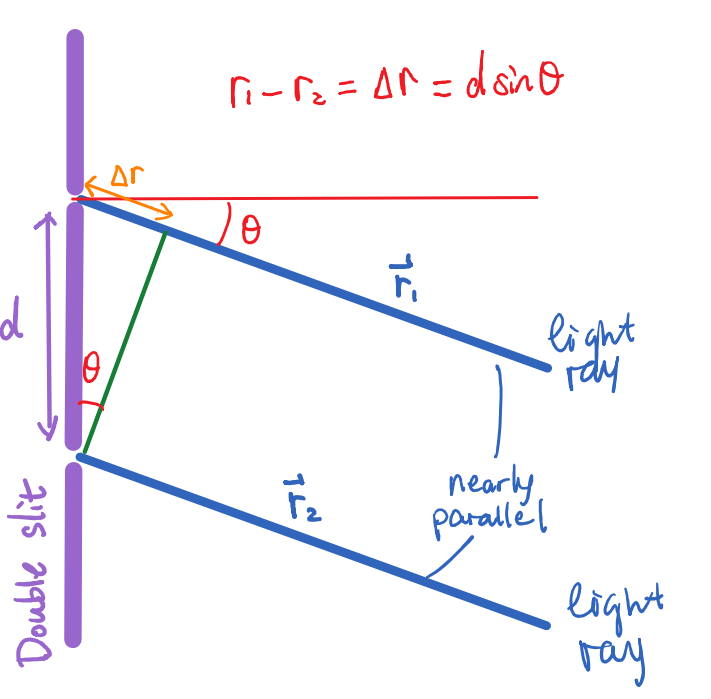
\includegraphics[scale=0.3]{slits.png}\qquad\qquad\qquad
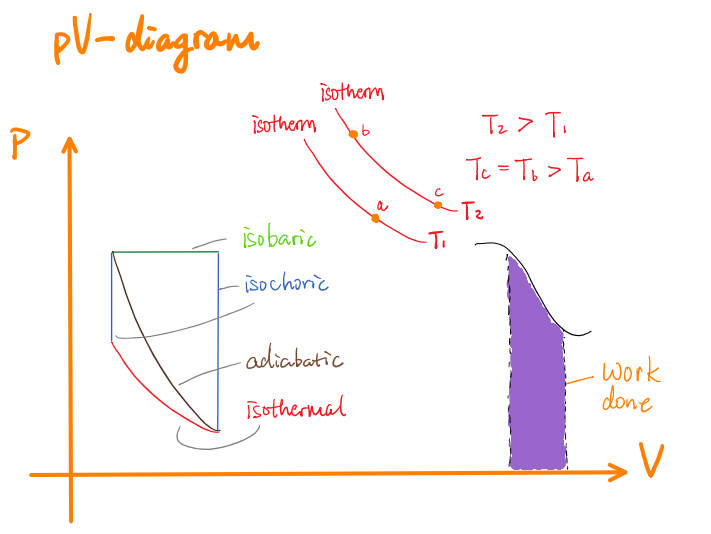
\includegraphics[scale=0.39]{thermo.png}
\end{center}


\begin{center}
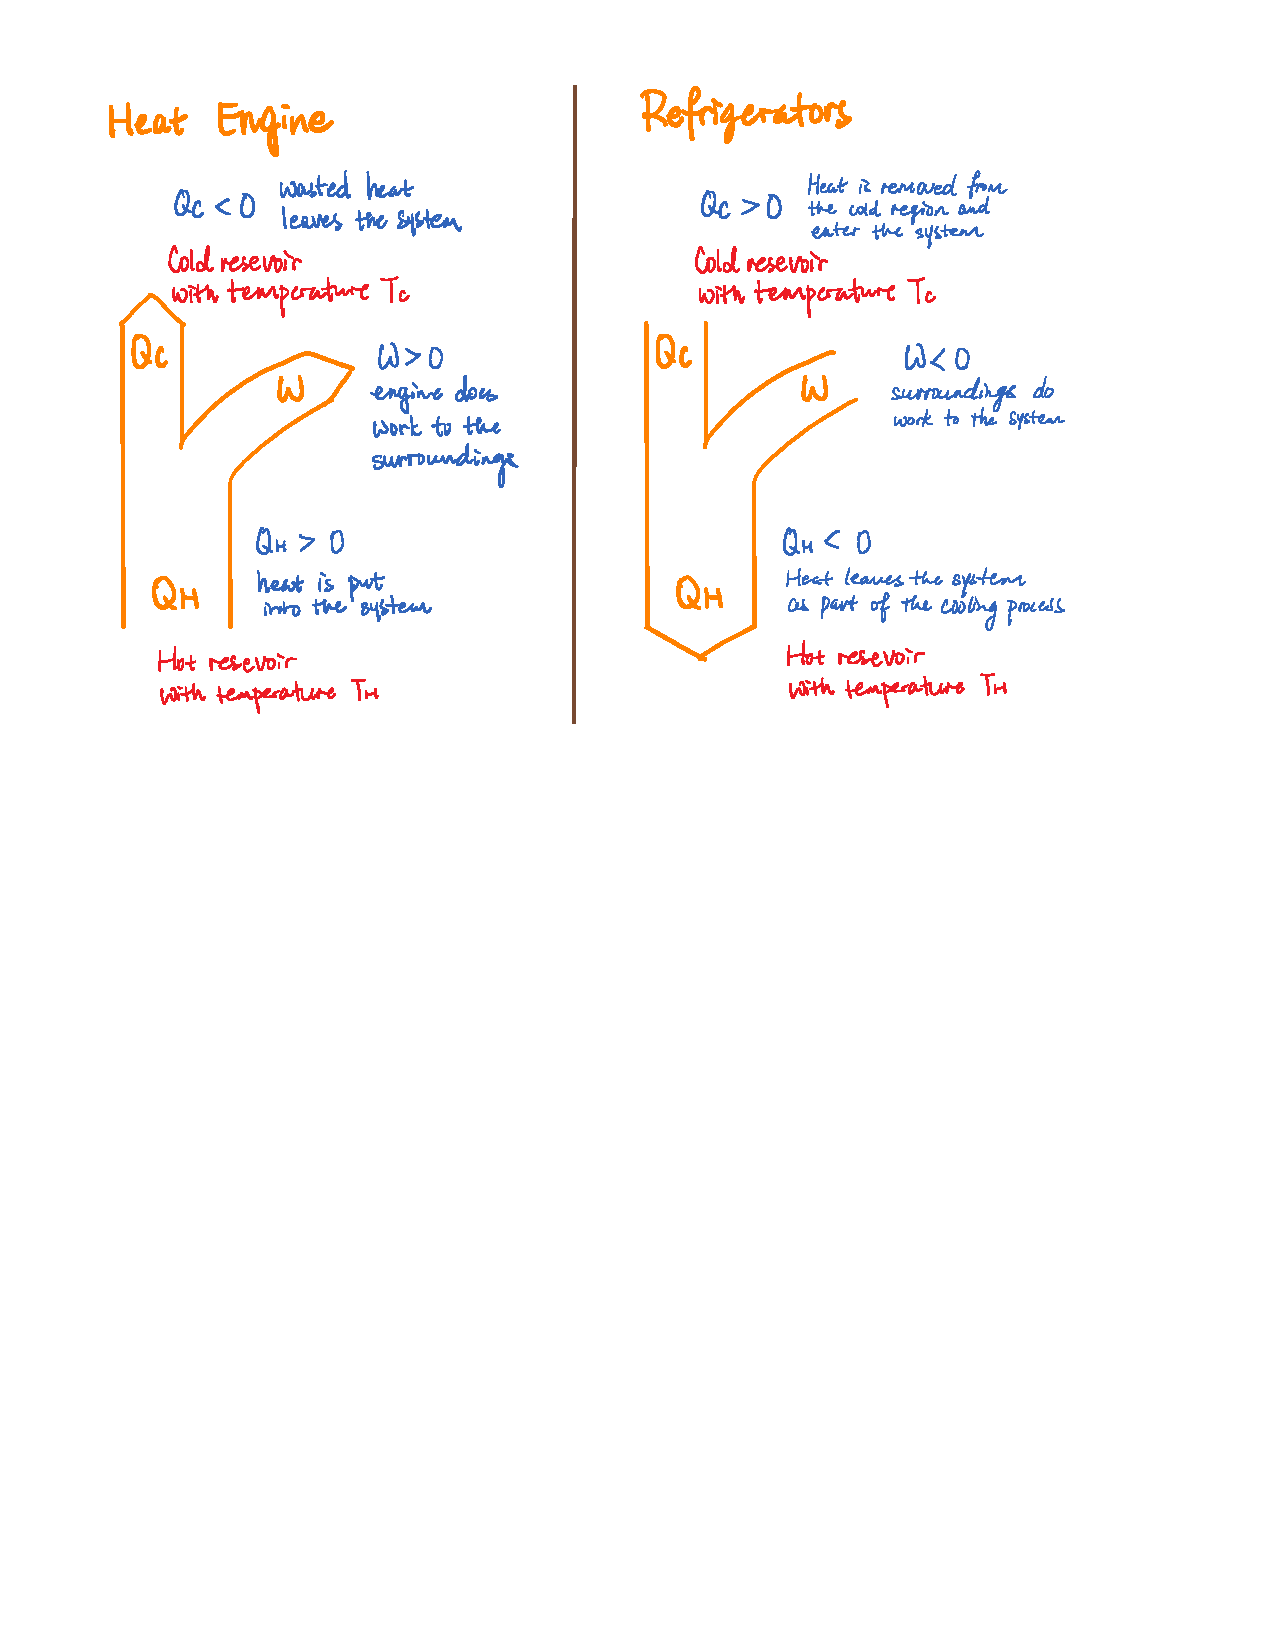
\includegraphics[scale=0.5]{cycles.pdf}
\end{center}


\end{document}
